\begin{figure}[ht]
	\centering
	\begin{subfigure}[t]{0.45\linewidth}
		\centering
		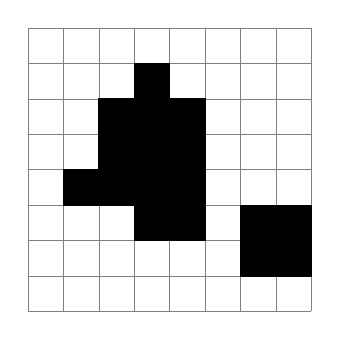
\begin{tikzpicture}[scale=0.45]
			\draw[help lines, step=1] (-4, -4) grid (4, 4);
			\foreach \x in {(-3, -1), (-2, -1), (-2, 0), (-2, 1), (-1, -2), (-1, -1), (-1, 0), (-1, 1), (-1, 2), (0, -2), (0, -1), (0, 0), (0, 1), (2, -3), (2, -2), (3, -3), (3, -2)}
				\filldraw[black] \x rectangle + (1, 1);
		\end{tikzpicture}
		\caption{Binary image.}
		\label{fig: openingbefore}
	\end{subfigure}
	\hfill
	\begin{subfigure}[t]{0.45\linewidth}
		\centering
		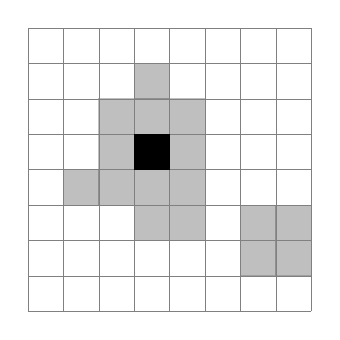
\begin{tikzpicture}[scale=0.45]
			\draw[help lines, step=1] (-4, -4) grid (4, 4);
			\foreach \x in {(-3, -1), (-2, -1), (-2, 0), (-2, 1), (-1, -2), (-1, -1), (-1, 0), (-1, 1), (-1, 2), (0, -2), (0, -1), (0, 0), (0, 1), (2, -3), (2, -2), (3, -3), (3, -2)}
				\filldraw[gray, opacity=0.5] \x rectangle + (1, 1);
			\foreach \x in {(-1, 0)}
				\filldraw[black] \x rectangle + (1, 1);
		\end{tikzpicture}
		\caption{Result of binary erosion of \ref{fig: openingbefore} with a $3 \times 3$ pixel structuring element. The light gray pixels are set to zero.}
		\label{fig: openingerosion}
	\end{subfigure}
	\vfill
	\begin{subfigure}[t]{0.45\linewidth}
		\centering
		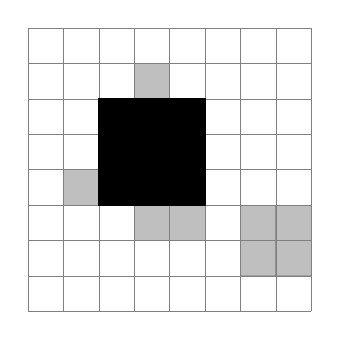
\begin{tikzpicture}[scale=0.45]
			\draw[help lines, step=1] (-4, -4) grid (4, 4);
			\foreach \x in {(-3, -1), (-1, -2), (-1, 2), (0, -2), (2, -3), (2, -2), (3, -3), (3, -2)}
				\filldraw[gray, opacity=0.5] \x rectangle + (1, 1);
			\foreach \x in {(-2, -1), (-2, 0), (-2, 1), (-1, -1), (-1, 0), (-1, 1), (0, -1), (0, 0), (0, 1)}
				\filldraw[black] \x rectangle + (1, 1);
		\end{tikzpicture}
		\caption{Binary dilation of the black pixel in \ref{fig: openingerosion} with a $3 \times 3$ pixel structuring element. The original image is displayed as light gray.}
		\label{fig: openingdilation}
	\end{subfigure}
	\hfill
	\begin{subfigure}[t]{0.45\linewidth}
		\centering
		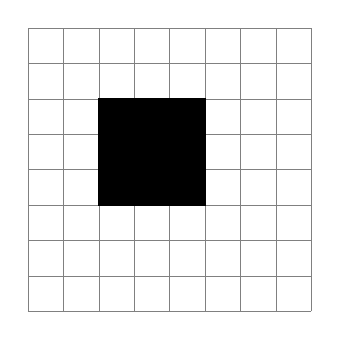
\begin{tikzpicture}[scale=0.45]
			\draw[help lines, step=1] (-4, -4) grid (4, 4);
			\foreach \x in {(-2, -1), (-2, 0), (-2, 1), (-1, -1), (-1, 0), (-1, 1), (0, -1), (0, 0), (0, 1)}
				\filldraw[black] \x rectangle + (1, 1);
		\end{tikzpicture}
		\caption{Result of opening of \ref{fig: openingbefore} with a $3 \times 3$ pixel structuring element. Outliers have been eliminated and edges have been smoothed.}
		\label{fig: openingafter}
	\end{subfigure}
	\caption{Example of binary morphological opening using a $3 \times 3$ pixel structuring element.}
	\label{fig: exampleopening}
\end{figure}